
\documentclass[main.tex]{subfiles}

\begin{document}

\chapter{Bond behavior}
\label{LEC:BondBehavior}

\paragraph{Outline:}
By saying that we want to capture the "material behavior" we mean that we realistically describe the relation \mnote{What is meant with material behavior}
between the strain and stress in a general material point. With the focus on a one-dimensional interface between two material components we can reduce this task to the relation between bond stress and slip. In Chapter~\ref{LEC:PullOut}, we simply assumed two shapes of the bond-slip relation, i.e. the constant bond-slip law for the stick-slip interface and a linear relation. The only reason we chose these two shapes was that for such laws, analytical solutions of the pullout boundary value problem can be found. However, the stick-slip interface cannot realistically describe the behavior of steel-concrete or FRP-concrete bond. 
In this chapter, we investigate more complex shapes of bond slip laws and their effect on the observed pullout response.

\paragraph{Addressed questions:}
\begin{itemize}
    \item 
How to characterize the bond.     \item 
What parameters influence the bond behavior? 
    \item 
What is a material law? What is a material point? 
    \item 
At which scale can we characterize a material behavior? 
    \item 
What is meant with a validity of a model?
\end{itemize}

\section{Generally nonlinear bond-slip law}
\label{SEC:gen_nonlinear_bs_law}

To solve a pullout problem for a generally nonlinear bond-slip law, we have to solve the initial boundary value problem numerically. We shall use a finite-element code implemented within the BMCS tool to study the behavior for two examples.
To make only a small step from the constant bond-slip law discussed in Chapter~\ref{LEC:PullOut} we modify this bond slip law only slightly in a way depicted in Fig.~\ref{FIGSourcesOfPlasticityHardening}. 
The shown modifications represent the increasing shear and decreasing shear during the sliding of the two surface over each other.
\begin{figure}[ht]
	\centering
  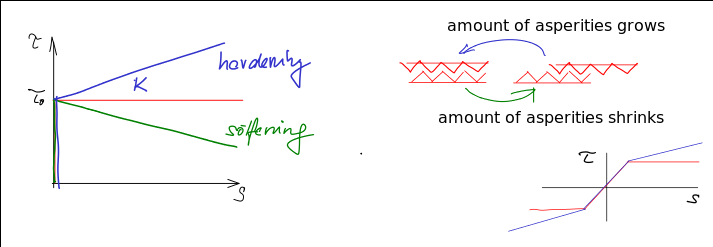
\includegraphics[trim={1mm 0mm 0mm 1mm},clip,width=0.7\textwidth]{drawings/plasticity_hardening_softenig.png}
	\caption{Structural interpretation of bond hardening and softening}
	\label{FIGSourcesOfPlasticityHardening}
\end{figure}

Even though analytical solutions for a piecewise-linear bond slip law have been derived it is more effective to apply general numerical finite-element solvers. 
Therefore, before proceeding to the study of the effect of the nonlinear bond-slip law on the pullout response, let us briefly touch the topic of the solution algorithm needed to solve the generally nonlinear problem. There are actually two questions that need to be addressed separately:
\begin{enumerate}
\item How to find the unknown displacement $u_\mathrm{f}$ satisfying the conditions of equilibrium, constitutive behavior and kinematics that we introduced in Sec~\ref{SEC:PullOutAnalyticalElasticMatrix} for a given level of load $P$ assuming linear bond-slip law? A very brief answer to this question is provided in Sec.~\ref{SEC:finite_element_pullout}. 
\item Based on the answer to question 1, how to define an iterative scheme that can handle non-linear type of bond-slip laws considered here? The principle approach to solving the nonlinear problem is show using an elementary type of function in Sec.~\ref{SEC:nonlinear_solver}.
\end{enumerate}
To provide an insight into the way how do the finite-element tools solve the problem an open implementation of the nonlinear solver, first in form of an open script that can be modified and tested.
This type of solver is provided in the BMCS tool suite to perform virtual tests and discuss the structural behavior later on. The same type of scheme is available in the most finite-element programs available on the market. The detailed explanation of the theoretical background is provided in the Master's courses on linear structural analysis focused on the theoretical background of the finite-element method and on the nonlinear structural analysis.

\begin{bmcsex}{Piecewise-linear bond slip laws}
{e31_piecewise_linear_bond_slip_law}
\paragraph{Task:} Use the corresponding jupyter notebook with the preconfigured pullout-model with piece-wise linear bond slip law to test the correspondence between the local bond law and the structural behavior. Cover the range of hardening and softening bond behavior.\\
\begin{center}
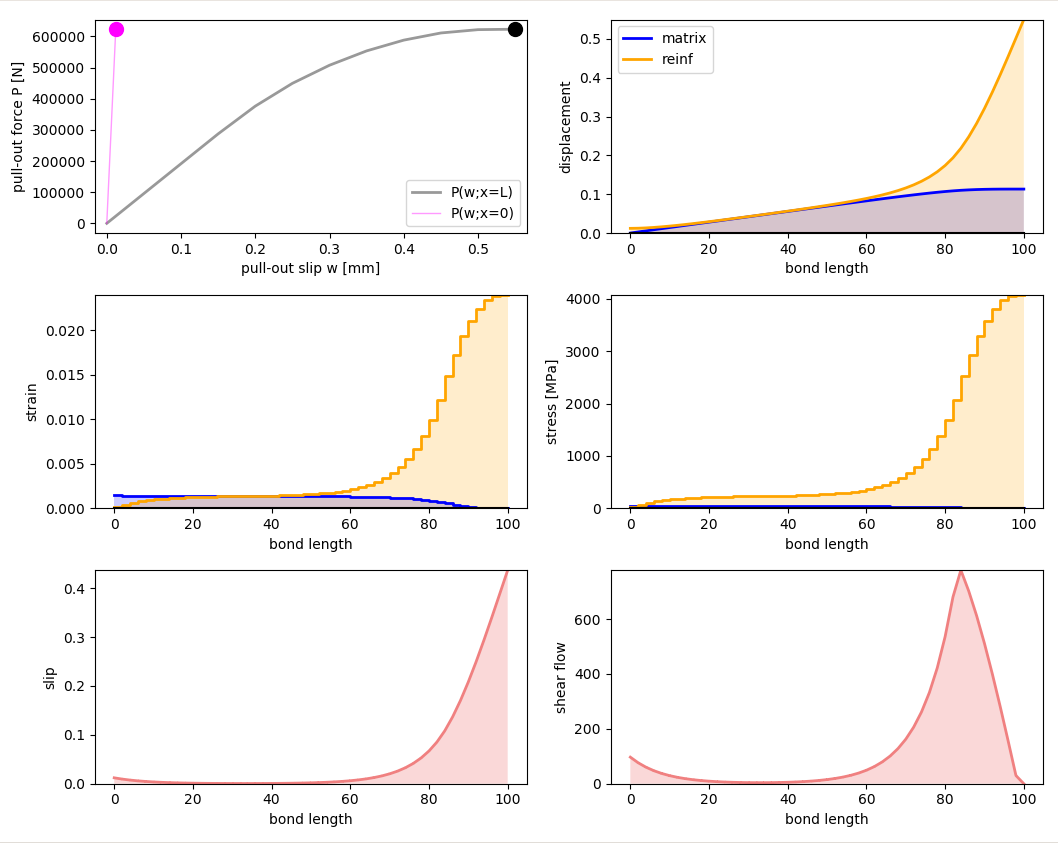
\includegraphics[width=0.7\textwidth]{fig/Lecture03/multilinear_bond.png}
\end{center}
\textbf{Task:} Answer the question: how does the response of the pullout curve evolve displayed for further increased pullout displacement $w = 0.15$~mm in the top left Figure ($P(w)$) and in the other diagrams showing the strain and stress state of the specimen?\\
\textbf{Task:} Answer the question: Based on the state variables (slip and shear stress along the bond zone) shown in the Figure: reconstruct the bond-slip law that was used in the simulation.
\end{bmcsex}

\section{Bond-slip law with hardening}
\label{SEC:bond-slip-hardening}

With the solution tool at hand let us return to the original question studying the effect of the hardening and softening in the bond-slip law. Assuming a bond slip law with hardening, 
To start with, let us return to the test results displayed in Fig.~\ref{fig_pull-out_rilem} of Sec.~\ref{Pullout_test_setup}. The tests were using the steel with the diameter $d=15$~mm with two embedded length. Thus, it should be possible to describe the pullout response of the two studied embedded lengths using the same bond-slip law.

If we can describe the two curves using an objective material model, i.e. a single bond-slip law, we might be able to predict the response in general and address the question of the anchorage length required for the particular type of a bar. Our first goals are the following:
\begin{description}
\item[Calibration] Choose one of the tests displayed in Fig.~\ref{fig_pull-out_rilem} (e.g. $L_\mathrm{b} = 5d$) and adjust the bond-slip law in such a way that the pullout curve roughly corresponds to the test response.
\item[Validation] Change the embedded length according to the other test, i.e. $L_\mathrm{b} = 10d$ and calculate 
the pullout curve. Check if it corresponds with the experimental response.
\item[Parametric study] Calculate the anchorage length, i.e. at which length does the bar yield or rupture?
\end{description}
This procedure introduces the notions of calibration, validation and parametric study that need to be explicitly distinguished when using models in combination with experimental data. Very often they are mixed up and it is not explicitly said if the modeled curve is a pure prediction, or if the parameters were adjusted to fit the experimental data.

The validation tells us to what extent is the model able to predict the behavior if we change the geometry or boundary conditions. It evaluates the quality and applicability of the model. 
If the model can reflect the essential effects included in the material behavior, it can be used to predict the response for changed parameters and boundary conditions. In our particular example, we might save experiments if we can trust the model that it can to some extent really substitute the experiment.

\begin{bmcsex}{Simulation of the RILEM pullout test}
{e32_rilem_pullout_test}
\paragraph{Question:} As an example of the three steps regarding the calibration, validation and parametric studies, 
the script provided on the server shows the bond-slip procedure using the finite-element simulator of the pullout within the BMCS tool suite. 
\begin{align}
\nonumber
d &= 16\;\mathrm{mm}, \;
E_\mathrm{f} = 210\;\mathrm{GPa}, \;
E_\mathrm{m} = 28\;\mathrm{GPa}, \\
\nonumber
A_\mathrm{f} &= \pi (\frac{d}{2})^2\;\mathrm{mm}^2, \; A_\mathrm{m} = (10d)^2 \;\mathrm{mm}^2, \;
p = \pi d
\end{align}
The bond-law roughly reproducing the standard RILEM test setup was identified in the form
\begin{center}
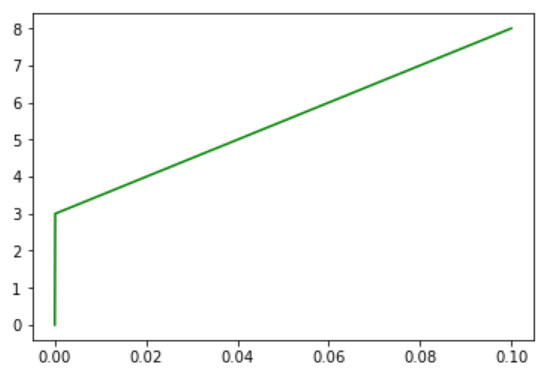
\includegraphics[width=8cm]{fig/Lecture03/bond_slip_rilem_test.png}\\
\end{center}
\paragraph{Task:} Use the bond-slip law to predict the other combinations of material parameters, i.e length of the bond zone $L_\mathrm{b} = 10d$ and different diameter $d = 28$~mm and $L_\mathrm{b} = 3d$.
\begin{center}
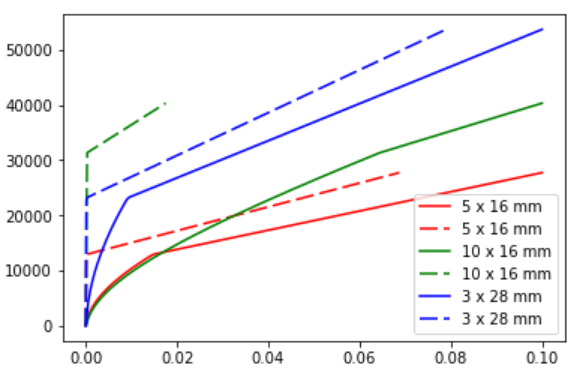
\includegraphics[width=10cm]{fig/Lecture03/pullout_rilem_test.png}
\end{center}
\paragraph{Task:}
Find out at which length $L_b$ the yielding of steel would start. question of anchorage length by repeated calculation of the pullout test with increasing anchorage length.
\end{bmcsex}

\subsection{How to determine the anchorage length in case of the constant bond-slip law?}
Let us consider the case of pull-out model with constant bond strength presented in Sec.~\ref{SEC:PullOutAnalytical} and qualitatively analyze the length-dependent pull-out response. Let us assume that the level of $\tau$, which is the only material parameter needed to characterize the bond-slip behavior, has been determined from a calibration experiment with embedded length $L_1$.
We can now make a prediction of the pull-out curves for embedded lengths $L_2$ and $L_3$ to obtain the respective pull-out curves depicted in Fig.~\ref{FIGPredictionConstantBond}. 
%
\begin{figure}[ht]
	\centering
  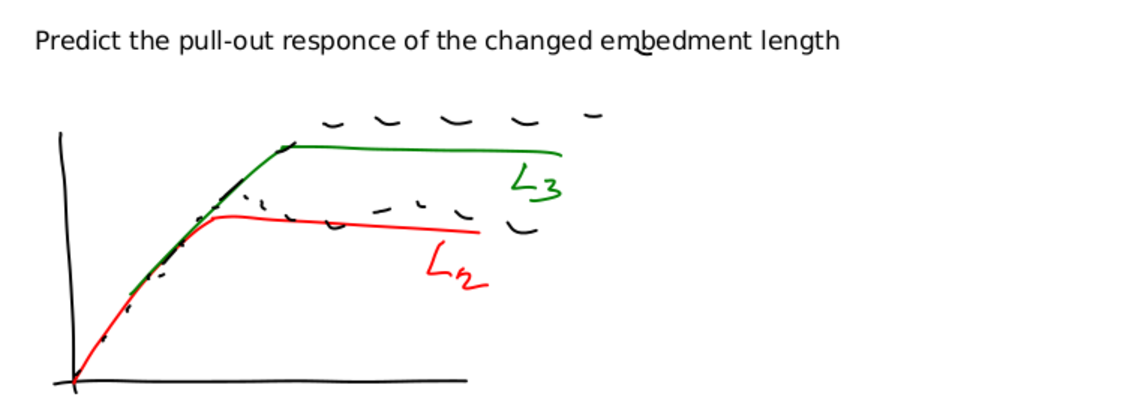
\includegraphics[width=0.7\textwidth]{drawings/prediction_constant_bond.pdf}
	\caption{Prediction of the constant bond model}
	\label{FIGPredictionConstantBond}
\end{figure}

The maximum achievable pull-out force of a test with an embedded length $L_\mathrm{b}$ is given as  
\begin{align}
\label{EQ:MaxEmbeddedLength}
P_{L} = \tau p L_\mathrm{b}
\end{align}
where $p$ denotes the perimeter, equal in all experiments. The force at  which the reinforcement attains the strength $\sigma_{\ifilam,\mathrm{mu}}$ and breaks is
\begin{align}
P_{\ifilam,\mathrm{mu}}  = \sigma_{\ifilam,\mathrm{mu}} A_\ifilam
\end{align}
so that the anchorage length obtained by setting $P_\tau = P_{\ifilam,\mathrm{mu}}$ reads 
\begin{align}
\label{EQ:ConstantBondAnchorageLength}
L_{\mathrm{anc}} = \frac{\sigma_{\ifilam,\mathrm{mu}} A_\ifilam }
{\tau p}.
\end{align}
The length-dependent maximum pull-out force is a bilinear function with a linear branch starting at zero and achieving the point
$[L_\mathrm{anc}, P_{\ifilam,\mathrm{mu}}$] as indicated in the right diagram of Fig.~\ref{fig_length_dependence}

\begin{figure}[ht]
	\centering
  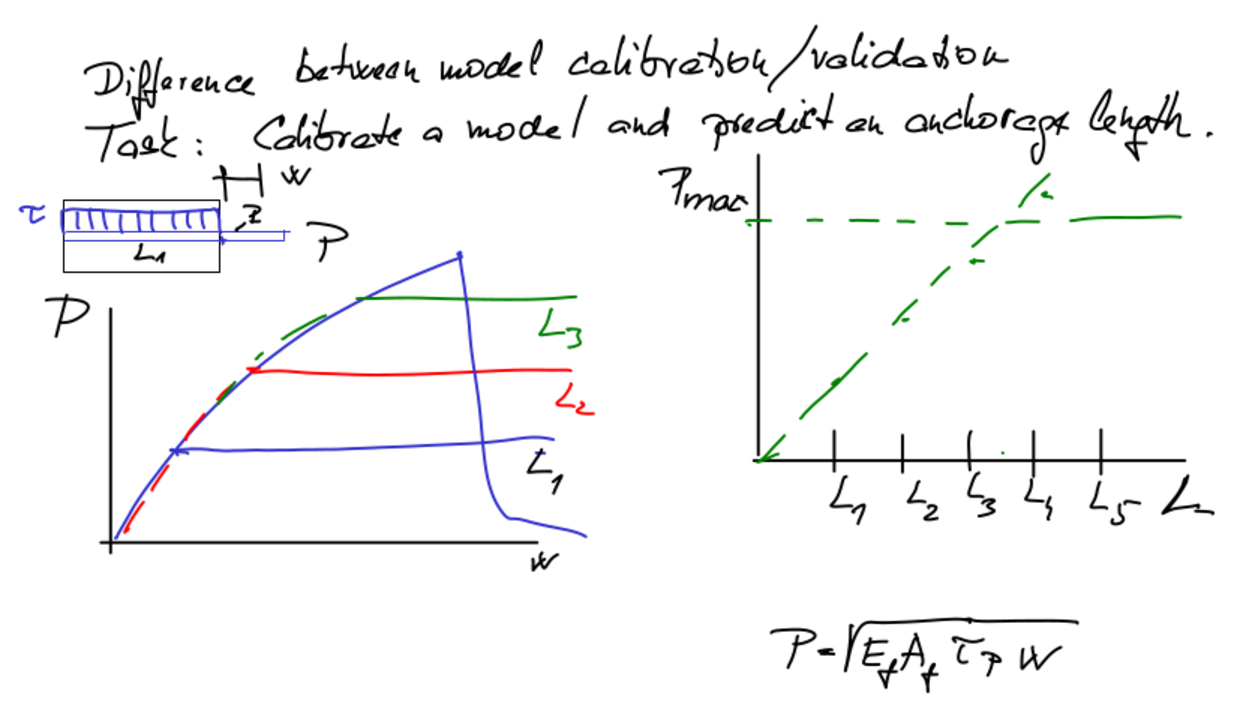
\includegraphics[width=0.8\textwidth]{drawings/lecture04-fig-plasticity-length-dependence.pdf}
	\caption{Length dependence}
	\label{fig_length_dependence}
\end{figure}
The simple bond-slip law allowed us to derive an explicit relation between the anchorage length, as a design parameter required for dimensioning of structures. This concept is  used in design equations. However, it must be used with care, since it is only valid for bond-slip laws that do not exhibit softening behavior as we shall document next.

%\section{Length dependent pull-out response for bond with hardening}

%An example study \ref{e43_po_hardening_length_dependence} shows the change of pullout response for increasing embedded length.


%\subfile{examples/e43_po_hardening_length_dependence/e43_po_hardening_length_dependence}

\section{Pullout problem for bond slip law with softening}
\label{SEC:bond_slip_softening}

A fundamentally different length-dependent behavior can be obtained if a bond-slip behavior exhibits softening. Assuming a bond-slip law with a peak bond stress $\tau_{\mathrm{mu}}$ at slip $s_{\mathrm{mu}}$ and decreasing shear stress for slip $s > s_{\mathrm{mu}}$ we shall now perform the same analysis of length dependency.

\begin{bmcsex}{Simulation of debonding between CFRP sheet and concrete}{e33_cfrp_and_concrete}
\paragraph{Question:} Considering FRP sheet used for strengthening, the bond-slip law with softening has been identified in a pullout test  \\
\begin{center}
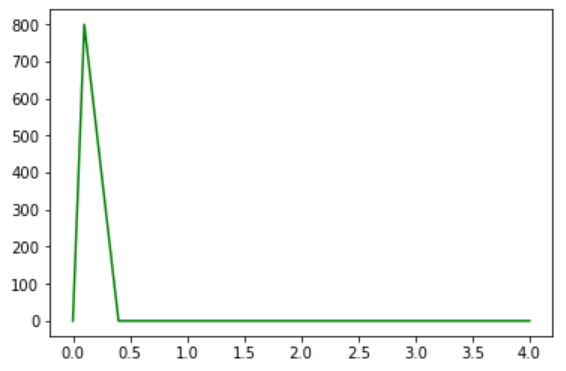
\includegraphics[width=8cm]{fig/Lecture03/bond_slip_frp_test.png}
\end{center}
The cross sectional parameters have been set to
\begin{align}
\nonumber
A_f = 16.67~\mathrm{mm}^2, \;
A_m = 1540.0~\mathrm{mm}^2, \;
E_f = 170000~\mathrm{MPa}, \;
E_m = 28000~\mathrm{MPa}
\end{align}
The perimeter $p = 1.0$ was considered that means the bond slip law was related to the whole width of the sheet.
\paragraph{Task:}
find out the length-dependent response. The pullout curves calculated for the bond legnth $L_\mathrm{b} \in (50,200)$~mm are obtained in the form\\
\begin{center}
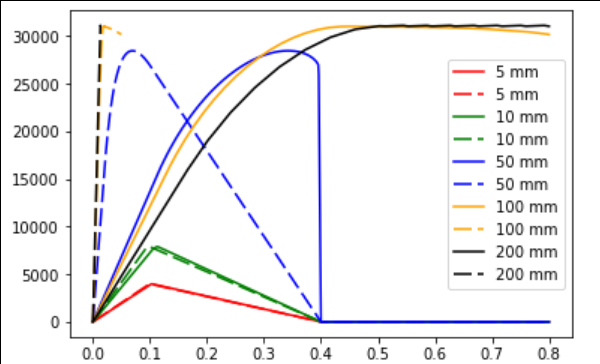
\includegraphics[width=10cm]{fig/Lecture03/pullout_frp_test.png}
\end{center}
\paragraph{Task:}
Answer the question: what is the anchorage length of the studied FRP?
\end{bmcsex}


\section{Finite element solution of the pullout problem}
\label{SEC:finite_element_pullout}

The provided code shows an application of these methods for the uniaxial discretization of the interface representing the embedded length. Every single point along the embedded length follows the behavior prescribed by the bond-slip law. The studies in the sequel will use linear finite elements representing the piecewise linear discretization of the embedded zone. Fig.~\ref{FIGLinearFiniteElements}.  
\begin{figure}[ht]
	\centering
  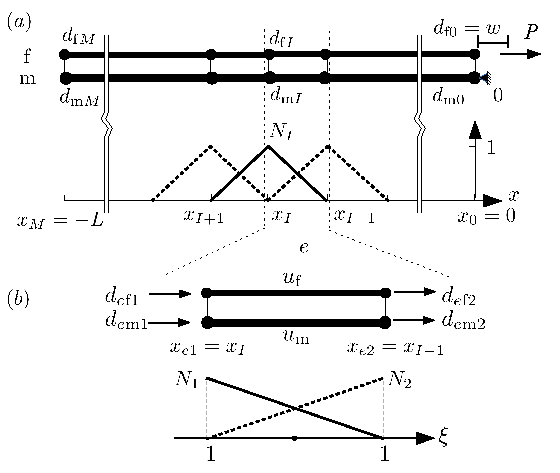
\includegraphics[width=0.7\textwidth]{fig/Lecture03/fe_i.pdf}
	\caption{Linear finite elements applied in the BMCS tool suite.}
	\label{FIGLinearFiniteElements}
\end{figure}
The displayed functions are non-zero only on a small subdomain. 
The sought displacement field of the reinforcement is approximated using the shape functions shown in Fig.~\ref{FIGLinearFiniteElements}a,
\begin{align}
 \label{eq:u_c_ansatz}
\nonumber
 u_\mathrm{f} = N_{I} \; d_{\mathrm{f}I}
\end{align}
with the index $I = 1,2,\dots, M$ representing the $I$-th node. 

% \begin{bmcsex}{Demonstration of the finite element solver}{ex_31_finite_elements}
% As we shall use the finite element solver in the sequel use the script provided \href{https://wiki.imb.rwth-aachen.de/do/view/IMB/Teaching/TeachExampleObj0007}{here} to 
% see how to setup the finite-element model and get the results.
% \end{bmcsex}

\section{Iterative solver for a general non-linear finite element simulation}
\label{SEC:nonlinear_solver}

To demonstrate the idea of a non-linear solver even in simple terms, let us consider a nonlinear function with just one unknown variable $f(u) = \bar{f}(t)$. 
Then, we assume to know the derivatives of the sought function with respect to the state variable $u$. The time stepping algorithm provides us a means how to travel through the space of state variables along an admissible path satisfying the governing equations. The director of the travel is the pseudo-time variable $t$.

In order to illustrate the concept, let us consider the simple function 
\begin{equation}
\bar{f}(t)= \mathrm{sin}(u)
\end{equation}
Think of this equation as the equilibrium requirement of our mechanical model. On the left hand side, there is the prescribed history of loads $\bar{f}(t)$. On the right hand side, the force of response of the structure. Now, for prescribed history on the right hand side $\bar{f}(t)$, we want to find the corresponding history of displacements satisfying the equilibrium $u(t)$. 

Of course, we might solve this equation just inverting the function to obtain the result
\begin{align}
u(t) = \arccos{f(t)}
\end{align}
but an inverse function is not available in a general case of a discretized structure. 
We thus pretend, that the inversion of the function $\sin(u)$ is not available and define the residuum of the problem as an implicit function
\begin{equation} \label{eq:residuum}
R = \mathrm{sin}(u) - \bar{f}(t) = 0.
\end{equation}
In a numerical code, the values of the function $\bar{f}(t)$ is given in incremental steps.
For each increment of $\bar{f}(t)$ an iteration loop must be performed to find the value of $u$ satisfying the residuum.

To get the numerical algorithm, we first expand the residuum using the first two terms of the Taylor series as
\begin{align}
R(u^{k+1},t) = R(u^{k},t) + \left.\frac{ \partial R(u) }{ \partial u }\right|_{u^k} \Delta u^{k+1} = 0.
\end{align}

In the considered case of $\sin{u}$, the derivative of the residuum with respect to $u$ is calculated as
\begin{equation}
\left.\frac{ \partial R(u) }{ \partial u } \right|_{u^k} = \mathrm{cos}(u^k)
\end{equation}

The iteration loop can then be obtained by solving the expanded residuum for the  increment of the displacement  $\Delta u^{k+1}$ as
\begin{equation}
\Delta u^{k+1} = - \left[ \left.\frac{ \partial R(u) }{ \partial u }\right|_{u^k} \right]^{-1} R(u^k)
\end{equation}
The new value of the  variable $u$ can be given as
\begin{equation}
u^{k+1} = u^k + \Delta u^{k+1} 
\end{equation}
The last two equations are repeated until the residuum is (almost) zero.
Graphical representation of this procedure is shown in Fig.~\ref{FIGNewtonAlgorithm} for a residuum given as function
$R(\varepsilon) := f(\varepsilon) - \hat{f} = 0$.
\begin{figure}[ht]
	\centering
  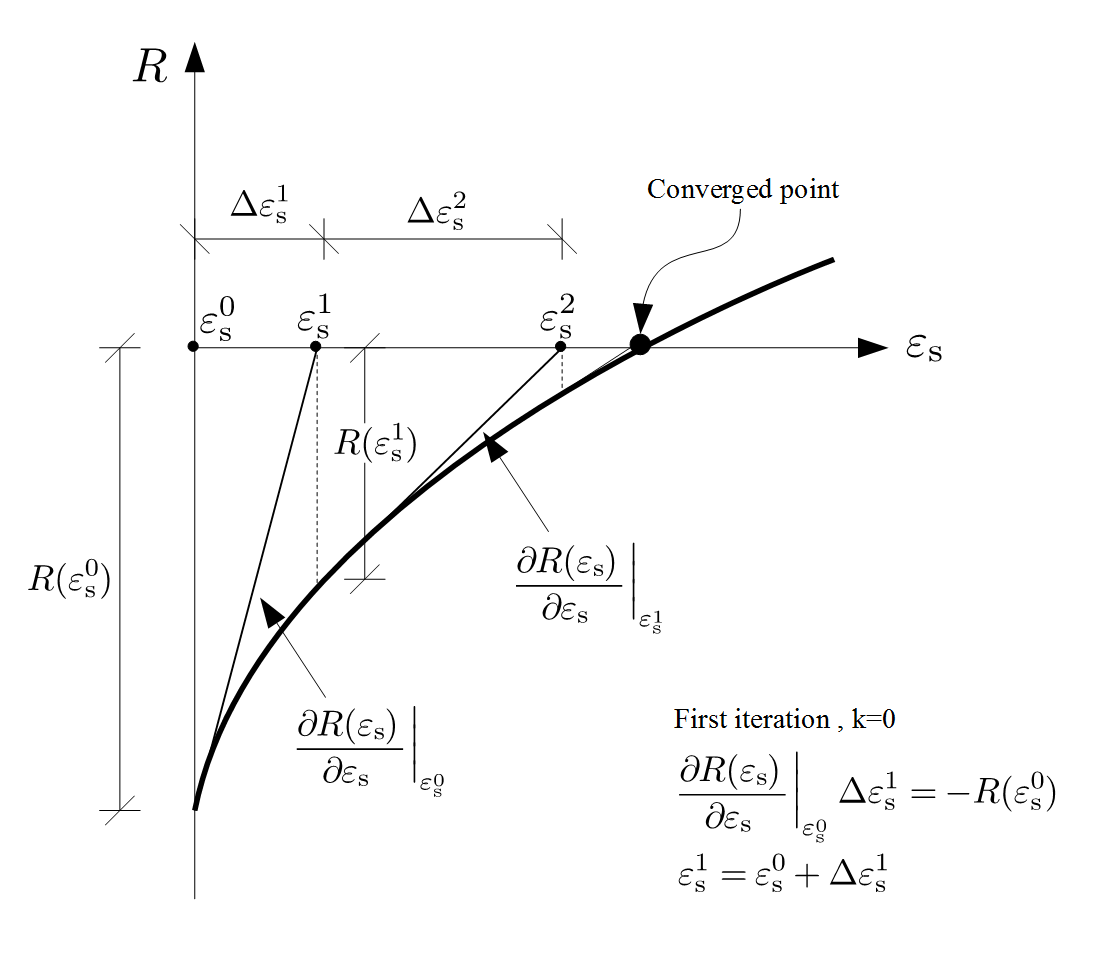
\includegraphics[width=0.7\textwidth]{fig/Lecture03/iterative_scheme.png}
	\caption{Nonlinear time stepping procedure following the Newton algorithm.}
	\label{FIGNewtonAlgorithm}
\end{figure}

This kind of incremental time-stepping procedure is used in the following examples that are solved either using the applications of the BMCS tool suite 
or using the ABAQUS, ANSYS, DIANA, ATENA, RFEM, InfoGraph, etc. Our goal is to illuminate the correspondence between the basic types of the bond-slip law and the observed pullout response. 

\begin{bmcsex}{Demonstration of the solution algorithm}{ex_32_nonlinear_scheme}
As an exercise, use the script provided on the server to 
see how the solution works.

The script discusses several types of responses represented by the three functions  $\sin{u}$, $u^2$ and $\sqrt{u}$. They indicate the issues that must be addressed in the non-linear finite element solver implementation.
\end{bmcsex}

\subsection{Related questions}
The models establish the basis for the consideration of further issues related to 
pull-out test and bond behavior.
\begin{itemize}
\item Plot a shape profile of a shear along the specimen at the maximum level of the pull-out force, how does it change during the loading
\item How does a shape of a shear flow correspond with a bond law?
\item How does the lateral pressure influence the bond behavior? 
\item What is the influence of lateral cracking?
\end{itemize}

\end{document}